\chapter{Problem description} \label{chap:problem_description}

This chapter introduces the optimization problem addressed in this thesis. Section~\ref{sec:competition_overview} provides a brief overview of the competition setting where the problem was initially assigned. In Section~\ref{sec:original_problem_statement}, the original problem statement is presented and explained in detail. Section~\ref{sec:further_insights_and_heuristics} explores additional insights and heuristics that we use to simplify the problem and improve solutions. Section~\ref{sec:datasets} describes the datasets provided with the problem. Finally, Section~\ref{sec:simulator} presents the custom simulator tool that we developed to evaluate solutions to the problem.

\section{Competition overview} \label{sec:competition_overview}

The problem we address in this thesis was originally assigned in the qualifying round of Google Hash Code 2021. Google Hash Code was a global team programming competition, running between 2014--2022, where teams of 2--4 competitors solved an optimization problem with the goal of achieving the best score in a limited time of 4 hours.

The usual solution procedure for our problem was as follows: Read the input data, create a trivial solution and write it to the output file in the specified format, and upload the solution to the evaluation system. The evaluation system not only displayed the score, but also some informative statistics, such as the number of cars that reached the finish before the deadline, the cars that arrived earliest and latest, the average cycle length of traffic lights at intersections, etc.
For some datasets, an interactive visualization of the evaluation process was also available, allowing to see the structure of a particular dataset. Although a local simulator was not needed to solve the problem, the manual upload of the solution to the evaluation system was slow and cumbersome and therefore not suitable for the use of efficient optimization algorithms.

Most teams were able to construct trivial solutions, which they then tried to improve by randomly changing the values. However, the best teams were able to write their own local simulator and use it to run multiple heuristics to get a better total score. Still, there was no time for anything more complex than a simple random search.

The total score was the sum of the scores of all 6 datasets (A--F). The first dataset (A) served as a ``toy problem'' mainly for debugging purposes, but the rest of the datasets were large enough for optimization. It should be noted that the distribution of points among the datasets is uneven, so the contestants mostly focused on the datasets with the highest possible score (D, F) and pragmatically skipped optimizing the rest (B, C, E).

\section{Original problem statement} \label{sec:original_problem_statement}

The full problem statement\footnote{\url{https://github.com/google/coding-competitions-archive/blob/main/hashcode/hashcode_2021_qualification_round.pdf}} is available in the Google Coding Competitions archive~\cite{google2023google}. Here we describe only important details for the reader.
In short, the task is as follows:
\begin{quote}
    \textit{Given a city plan describing intersections and streets and cars with planned paths through the city, optimize the schedule of traffic lights to minimize the total amount of time spent in traffic, and help as many cars as possible reach their destination before a specified deadline.}
\end{quote}
In terms of graph theory, the city plan is a \textit{directed graph}. The intersections are \textit{vertices} and the streets are \textit{directed edges} (see Figure~\ref{fig:hashcode_city_plan}). The planned path for each car is indeed a \textit{path} in this graph because it has a different start and end, and no intersection is repeated.

\begin{figure}
    \centering
    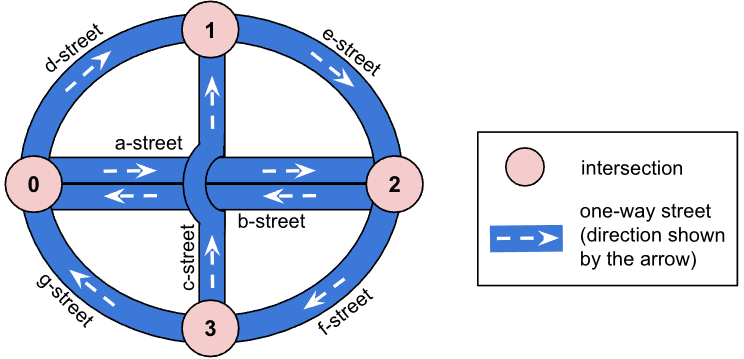
\includegraphics[width=\linewidth]{img/hashcode/figure1.png}
    %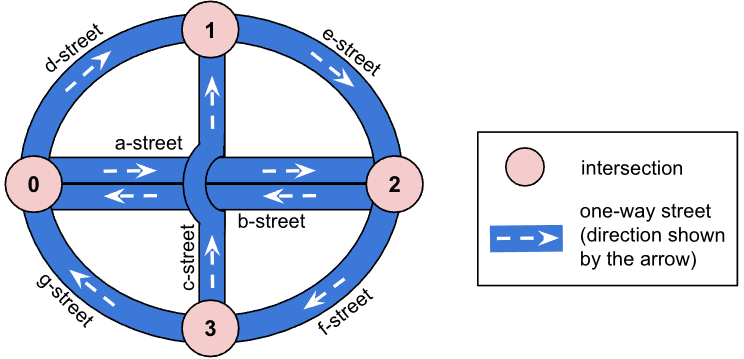
\includegraphics[width=.8\linewidth]{img/hashcode/figure1.png}
    \caption[Example of a city plan]{
        Example of a city plan \cite{google2023google}.
    }
    \label{fig:hashcode_city_plan}
\end{figure}

\subsection{Streets and intersections}

In the city, we have a set of intersections
$I$, where $2 \leq \abs{I} \leq 10^5$,
and a set of streets
$S \subseteq \{(u, v) | u,v \in I \land u \neq v\}$, where $2 \leq \abs{S} \leq 10^5$.
Each street $s \in S$ is a unique one-way connection between two different intersections $u$, $v$; two distinct streets in opposite directions between the same two intersections $(u, v)$, $(v, u)$ are allowed. Each street $s \in S$ has a fixed time $l(s) \in \mathbb{N}_+$ that it takes a car to get from the beginning to the end of the street, independently of the other cars on the street.
Each intersection $i \in I$ has a set of incoming streets $S_i^+ \subset S$, where $|S_i^+| \geq 1$, and a set of outgoing streets $S_i^- \subset S$, where $|S_i^-| \geq 1$; thus each intersection has at least one incoming street and at least one outgoing street.

\subsection{Traffic lights and schedules}

In each intersection $i \in I$, there is a traffic light at the end of each \textit{incoming} street $s^+ \in S_i^+$. The traffic light has two states---green and red. Green means the cars from this street can pass through the intersection and continue to any \textit{outgoing} street $s^- \in S_i^-$ in their path. Red means the cars must stop until the light turns green again. At most one traffic light can be green at each intersection at any time.

When the light is red, cars arriving at the end of a street queue up and wait for the light to turn green. The queue does not take up any space and does not change the distance cars have to travel. When the light is green, one car can pass through an intersection every second. Passing through an intersection, i.e., moving from the end of an incoming street to the beginning of an outgoing street, takes no additional time.

For each intersection $i \in I$, we can set a traffic light schedule. This schedule determines the order and duration of green light for the incoming streets of the intersection. The schedule repeats in a cycle until the end of the simulation (see Figure~\ref{fig:hashcode_traffic_lights}). Each street can appear at most once in the schedule. If a street is not included in the schedule, it is red the whole time, and any waiting cars are blocked. By default, intersections have no schedule and all streets are red.

% https://tex.stackexchange.com/questions/69869/image-taking-up-full-page
\begin{figure}[ht] % h = here, t = top, p = page of floats
    \centering
    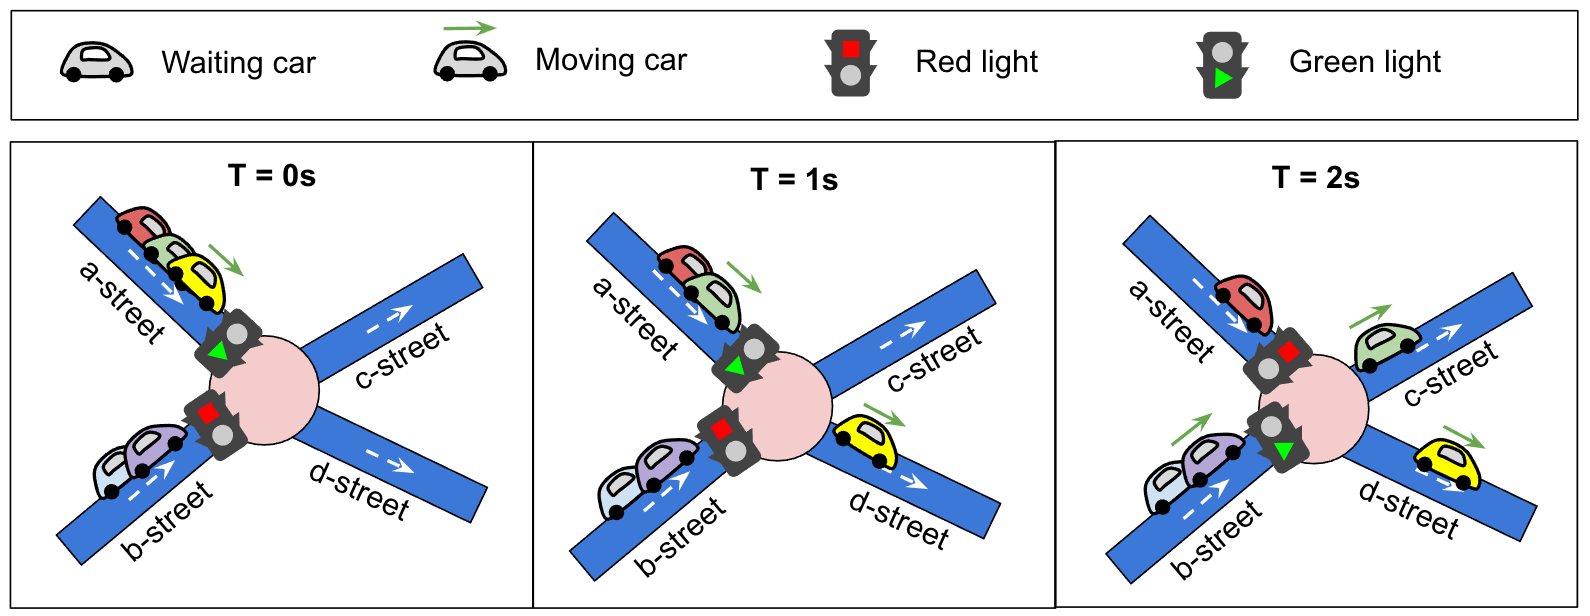
\includegraphics[width=\linewidth]{img/hashcode/figure2-abc.png}
    % 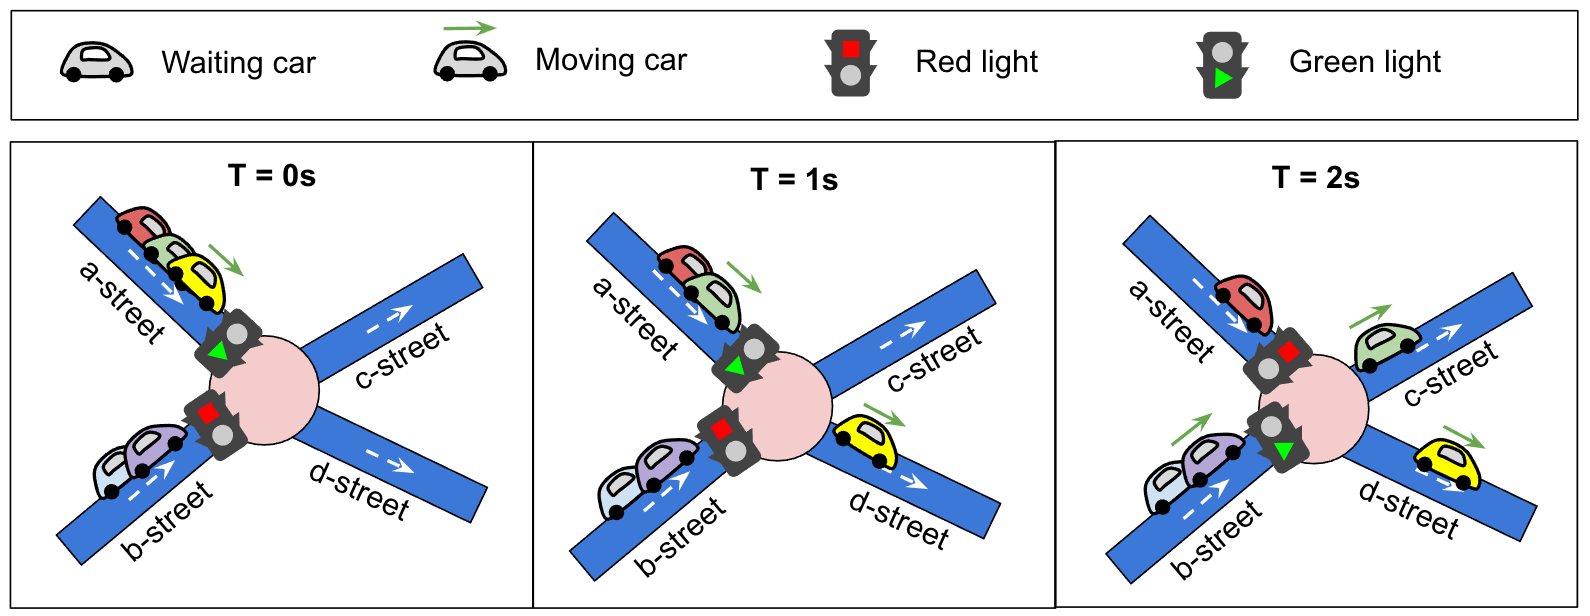
\includegraphics[width=.8\linewidth]{img/hashcode/figure2-abc.png}
    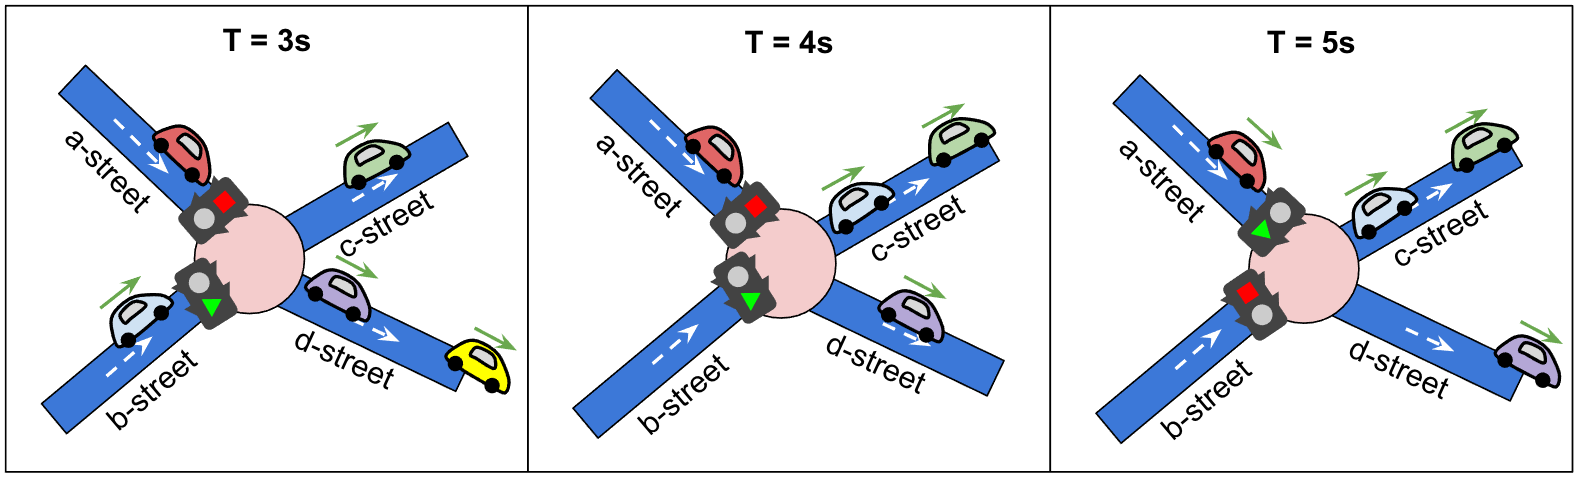
\includegraphics[width=\linewidth]{img/hashcode/figure2-def.png}
    % 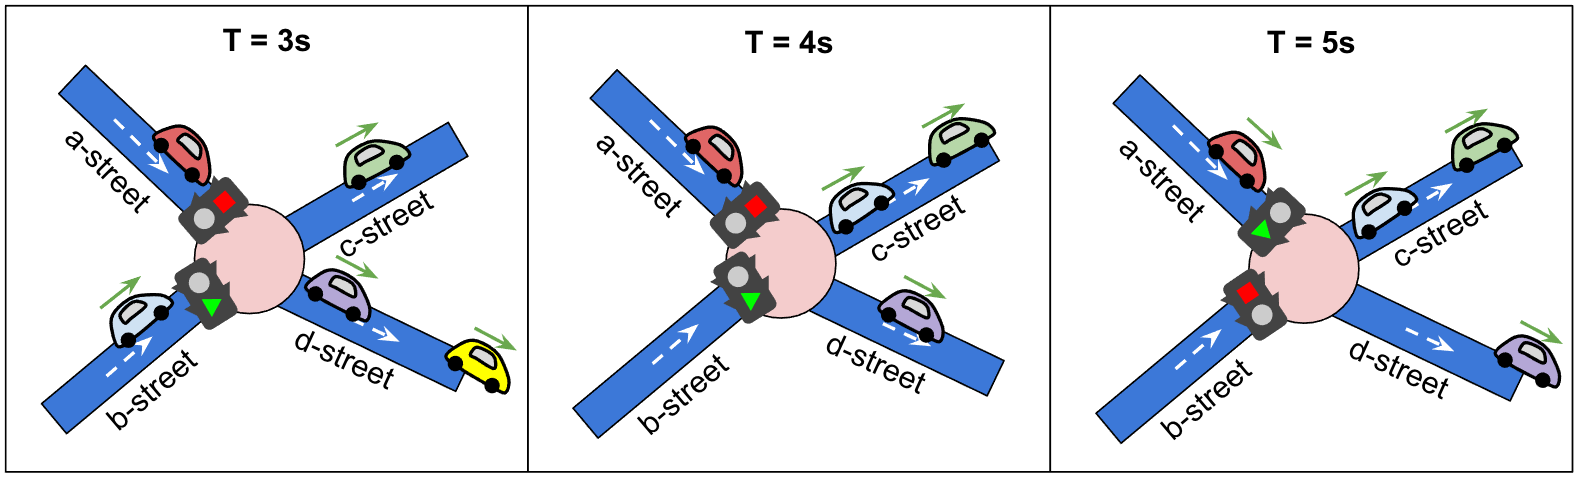
\includegraphics[width=.8\linewidth]{img/hashcode/figure2-def.png}
    \caption[Example of a traffic light schedule]{
        This figure shows how the traffic light schedule works for an intersection with two incoming streets \cite{google2023google}.
        The schedule is as follows: First \textit{a-street} for $2$ seconds, then \textit{b-street} for $3$ seconds.
        We can see the first two cars from \textit{a-street} pass in the first two seconds, then the green light switches to \textit{b-street} for three seconds,
        allowing the two cars from \textit{b-street} pass. The last car from \textit{a-street} waits till the beginning of the next cycle and then passes.
    }
    \label{fig:hashcode_traffic_lights}
\end{figure}

\subsection{Cars}

Furthermore, we have a set of cars $C$, where $1 \leq \abs{C} \leq 10^3$. Each car $c \in C$ has a given path through the city. The path is a sequence of streets the car has to drive through. The number of streets in the path is limited: $\forall c \in C \;\; 2 \leq \abs{\bm{p_c}} \leq 10^3$. No intersection or street can be repeated in the path.

At the beginning of the simulation, all cars are at the end of the first street in their path. They either wait if the light is red or are ready to move if the light is green. If more cars start at the end of the same street, they queue up according to their IDs in the input file (see Figure~\ref{fig:hashcode_street}). When a car reaches the end of the last street in its path, it is immediately removed from the street.

\begin{figure}[ht] % h = here, t = top, p = page of floats
    \centering
    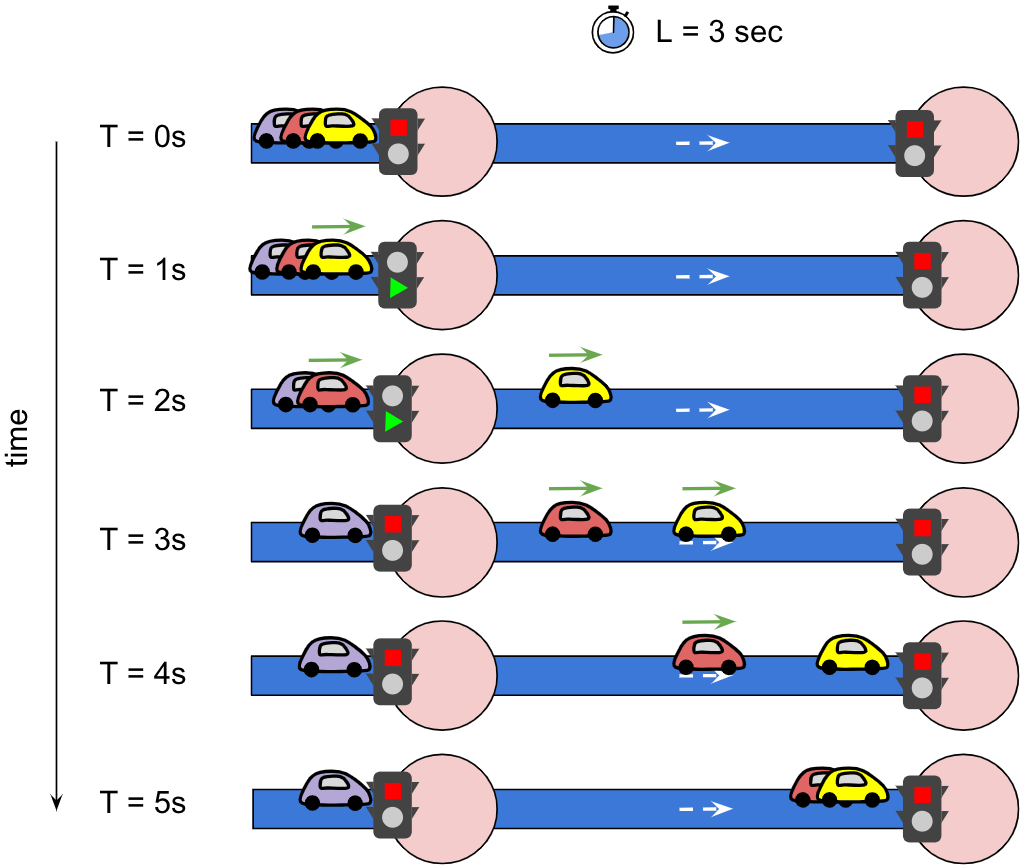
\includegraphics[width=\linewidth]{img/hashcode/figure3.png}
    %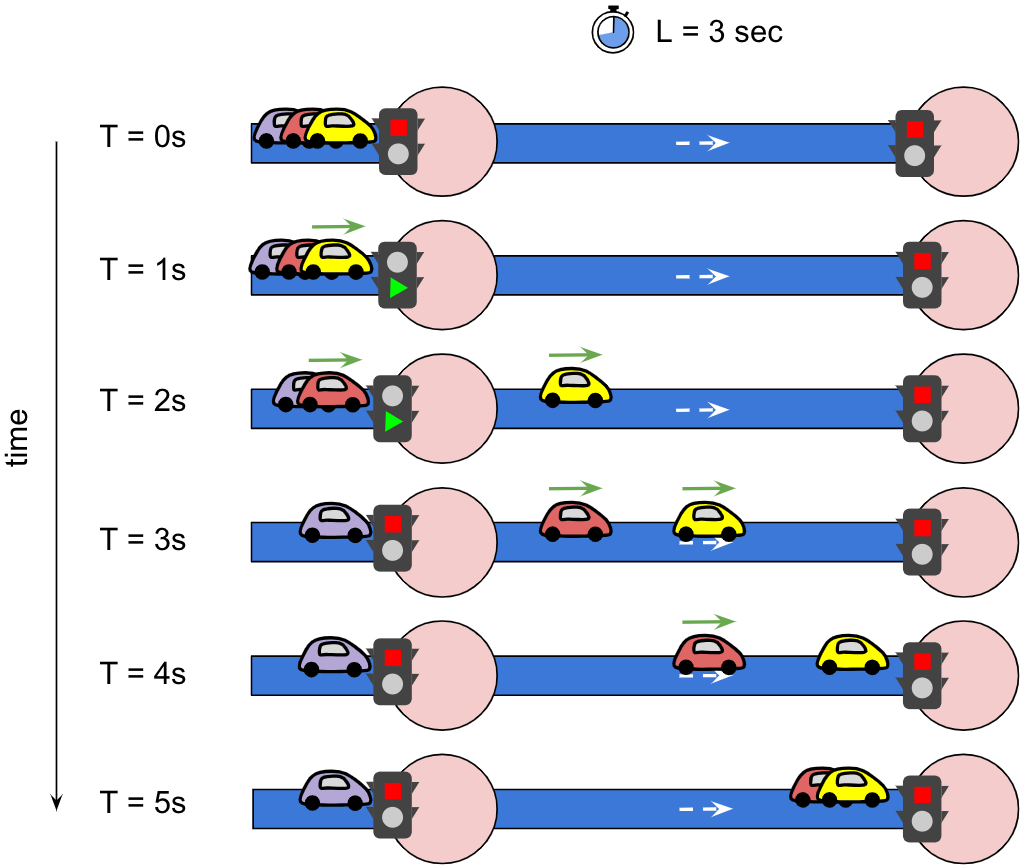
\includegraphics[width=.8\linewidth]{img/hashcode/figure3.png}
    \caption[Example of cars driving through a street]{
        This figure shows the first five seconds of a~simulation \cite{google2023google}.
        For simplicity, only one street is shown in the figure; when the light is red for this street, it is green for another street in the same intersection.
        When the light turns green at $T=1s$, the first (yellow) car immediately passes the intersection and moves to the next street, reaching the end of the street at $T=4s$.
        At $T=2s$, the light is still green, so the second (red) car passes the intersection and moves to the next street, reaching the end of the street at $T=5s$.
        From $T=3s$ to $T=5s$, the light is red, so the third (purple) car cannot pass the intersection and has to wait for the next cycle.
    }
    \label{fig:hashcode_street}
\end{figure}

\newpage

\subsection{Score}

The score of a solution is determined as follows: Let $\bm{\theta}$ denote the traffic light schedules. Given a duration of the simulation $\mathrm{D}$ in seconds, where $1 \leq \mathrm{D} \leq 10^4$, and a fixed bonus for reaching the destination $\mathrm{F}$, where $1 \leq \mathrm{F} \leq 10^3$, let $t(c; \bm{\theta}) \in \mathbb{N}$ be the time a car $c \in C$ reaches the destination. The $score$ of a car $c$ is defined as
\begin{equation}
    score(c; \bm{\theta}) =
    \begin{cases}
        \mathrm{F} + (\mathrm{D} - t(c; \bm{\theta})), & \text{if $t(c; \bm{\theta}) \leq \mathrm{D}$}, \\
        0, & \text{otherwise}.
    \end{cases}
\end{equation}
The $SCORE$ of a solution $\bm{\theta}$ is defined as
\begin{equation}
    SCORE(\bm{\theta}) = \sum_{c \in C} score(c; \bm{\theta}).
\end{equation}

\section{Further insights and heuristics} \label{sec:further_insights_and_heuristics}

In this section, we introduce some additional terms and heuristics for the problem. These are our own observations and are not part of the original problem statement. Thanks to these heuristics, we can simplify the solution creation, achieve better scores, and reduce the number of parameters to optimize.

\paragraph{Used and unused streets} \textit{Unused street} is a street that is either not used by any car at all or it is the final destination of all cars that use it (i.e. traffic light for this street is not needed). \textit{Used street} is a street that is used by at least one car and is not the final destination of at least one car that uses it.

\paragraph{Used and unused intersections} \textit{Unused intersection} is an intersection where all incoming streets are unused streets. \textit{Used intersection} is an intersection with at least one used incoming street.

% https://tex.stackexchange.com/questions/32160/new-line-after-paragraph
\paragraph{Heuristic 1: Remove unused intersections and unused streets} \label{para:heuristic_1} \mbox{} \\
Remove unused intersections and unused streets from used intersections when creating initial schedules. They contribute nothing and can only worsen the score. \\

This heuristic is an obvious one; unused intersections are never used and only add unnecessary complexity. Unused streets prolong the traffic light cycle for the whole intersection, which very frequently leads to longer waiting times and thus a lower score. Now, let us move on to some less obvious insights.

\paragraph{Trivial and non-trivial intersections} \textit{Trivial intersection} is an intersection with exactly one used incoming street. \textit{Non-trivial intersection} is an intersection with two or more used incoming streets.

\paragraph{Blocked streets and blocked intersections} \textit{Blocked street} is an unscheduled street or a street with a green light scheduled for 0 seconds. \textit{Blocked intersection} is an intersection with no schedule or with all incoming streets blocked.

\paragraph{Heuristic 2: Fix the schedule for trivial intersections, optimize only non-trivial schedules} \label{para:heuristic_2}
Trivial intersections do not require optimization; their schedule can be fixed by giving a green light to the only used incoming street for the entire duration. Only the schedules of non-trivial intersections need to be optimized. This can substantially reduce the number of optimized parameters. \\

This heuristic is not straightforward, so let us think about it in more detail. For trivial intersections, we have two meaningful schedule options:
\begin{enumerate}
    \item Keep the light green the whole time.
    \item Keep the light red the whole time, effectively blocking all cars there.
\end{enumerate}
Empirically speaking, the vast majority of trivial intersections should be kept green anyway, otherwise many cars would not be able to reach their destination at all.
Furthermore, we argue that we can omit the second option because we can achieve a similar result in a different way. Suppose that blocking a particular trivial intersection improves the score. This means that there must be a problematic car passing through this intersection. However, the problematic car must eventually reach some non-trivial intersection via a street, and this street can still be blocked during optimization. We therefore leave this up to the optimization algorithm, hoping that it explores this option if it is indeed beneficial.

As previously mentioned, this smart heuristic is important because it allows us to focus only on the non-trivial intersections and simplifies the optimization process. To put it into perspective, approximately $80 \%$ of used intersections in dataset B are trivial, $60 \%$ in dataset C, and $50 \%$ in dataset E. This enables us to skip optimizing thousands of parameters.

\section{Datasets} \label{sec:datasets}

In this section, we briefly describe all datasets provided with the problem. The datasets vary in the size and structure of their city plans. We define the size of a dataset as the number of parameters we need to optimize.
The number of parameters for each dataset is twice the total number of used streets in non-trivial intersections (one parameter for the order and one for the green light duration). Note that this is only one way to compare the datasets, and it does not account for the actual paths cars must take or how convoluted those paths may be.

\begin{figure}[h]
    \centering
    % 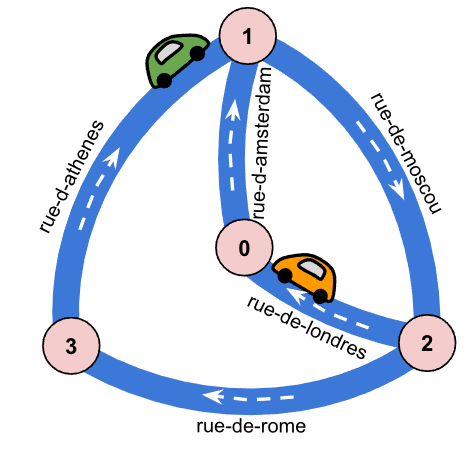
\includegraphics[width=\linewidth]{img/hashcode/figure5.png}
    % 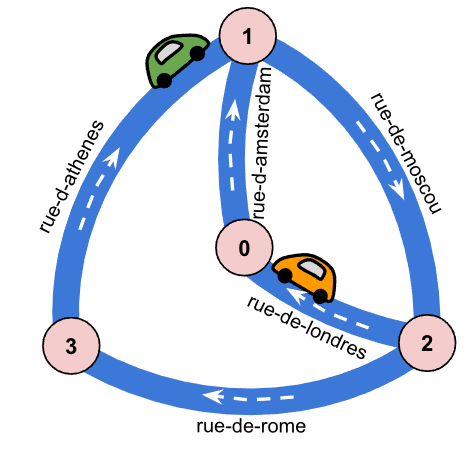
\includegraphics[width=.6\linewidth]{img/hashcode/figure5.png}
    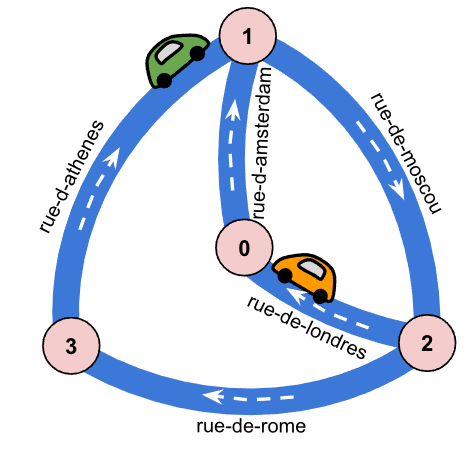
\includegraphics[width=.5\linewidth]{img/hashcode/figure5.png}
    \caption[Visualization of dataset A]{
        Visualization of dataset A \cite{google2023google}.
    }
    \label{fig:hashcode_dataset_a}
\end{figure}

\paragraph{A - An example: 4 parameters} Simple toy problem dataset used for debugging (see Figure~\ref{fig:hashcode_dataset_a}).

\paragraph{B - By the ocean: 5,974 parameters} Dataset based on a real city plan of Lisbon, Portugal (see Figure~\ref{fig:hashcode_dataset_b}).

\paragraph{C - Checkmate: 14,008 parameters} Dataset with a chessboard-like pattern and regular structure of intersections and streets (see Figure~\ref{fig:hashcode_dataset_c_e}).

% https://codeforces.com/blog/entry/88188#comment-765574
\paragraph{D - Daily commute: 167,748 parameters} By far the largest dataset with a challenging-to-navigate network from the \textit{Barabási-Albert} \cite{albert2002statistical} distribution.

\paragraph{E - Etoile: 1,386 parameters} Nicknamed \textit{Etoile}\footnote{\textit{Étoile} means star in French.}, this dataset is a one big star, meaning there is one very important intersection in the middle with hundrets of incoming streets (see Figure~\ref{fig:hashcode_dataset_c_e}).

\paragraph{F - Forever jammed: 10,002 parameters} Medium sized dataset but again with a complex network difficult to optimize.

\begin{figure}[h]
    \centering
    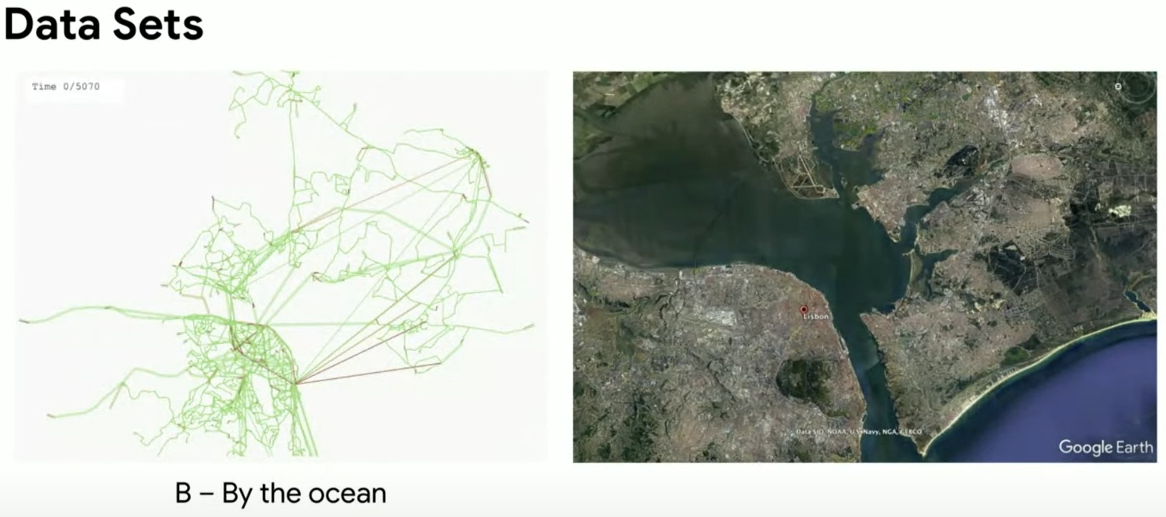
\includegraphics[width=\linewidth]{img/screenshots/hashcode_datasets_b.png}
    % 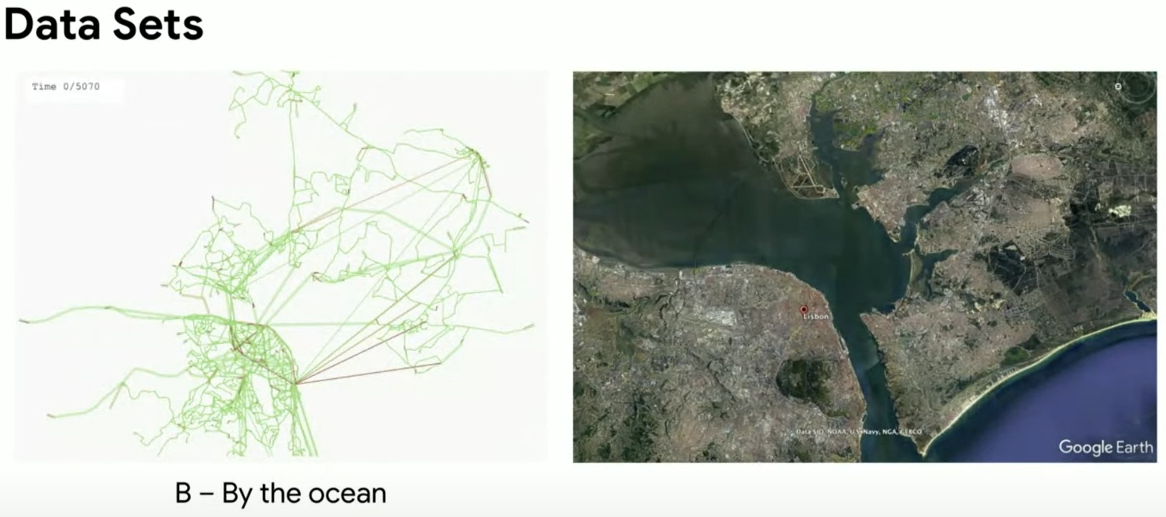
\includegraphics[width=.8\linewidth]{img/screenshots/hashcode_datasets_b.png}
    \caption[Visualization of dataset B]{
        Dataset B based on the real data of Lisbon on the right\footnotemark.
    }
    \label{fig:hashcode_dataset_b}
\end{figure}

\footnotetext{Screenshot from \href{https://www.youtube.com/watch?v=YPOVd-hQUjA}{Hash Code 2021: Online Qualification Round Livestream}.}

\bigskip

As mentioned in Section~\ref{sec:competition_overview}, each dataset yields an absolute score within a different range. To compare the performance across all datasets, we normalize the scores to a 0--1 scale, where 0 represents a baseline solution (see Section~\ref{sec:initial_schedules} for details), and 1 corresponds to the maximum known score\footnote{See the maximum known scores \href{https://github.com/sagishporer/hashcode-2021-qualification\#score}{here}.} for the dataset. Note that the baseline is already a good solution, so there may be limited room for improvement---for example, in dataset B.

\begin{figure}[h]
    \centering
    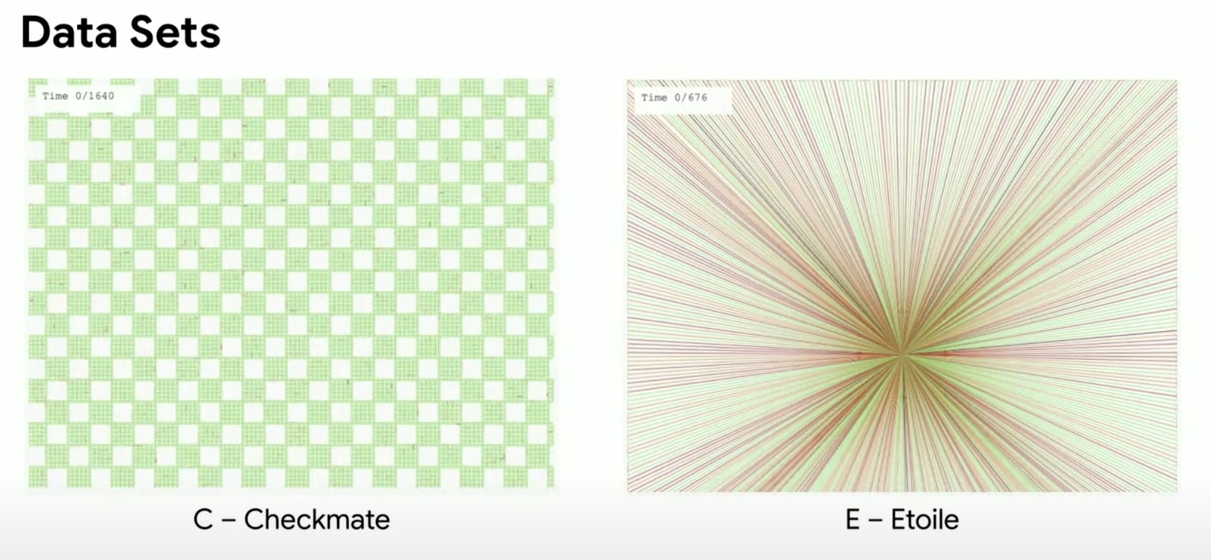
\includegraphics[width=\linewidth]{img/screenshots/hashcode_datasets_c_e.png}
    % 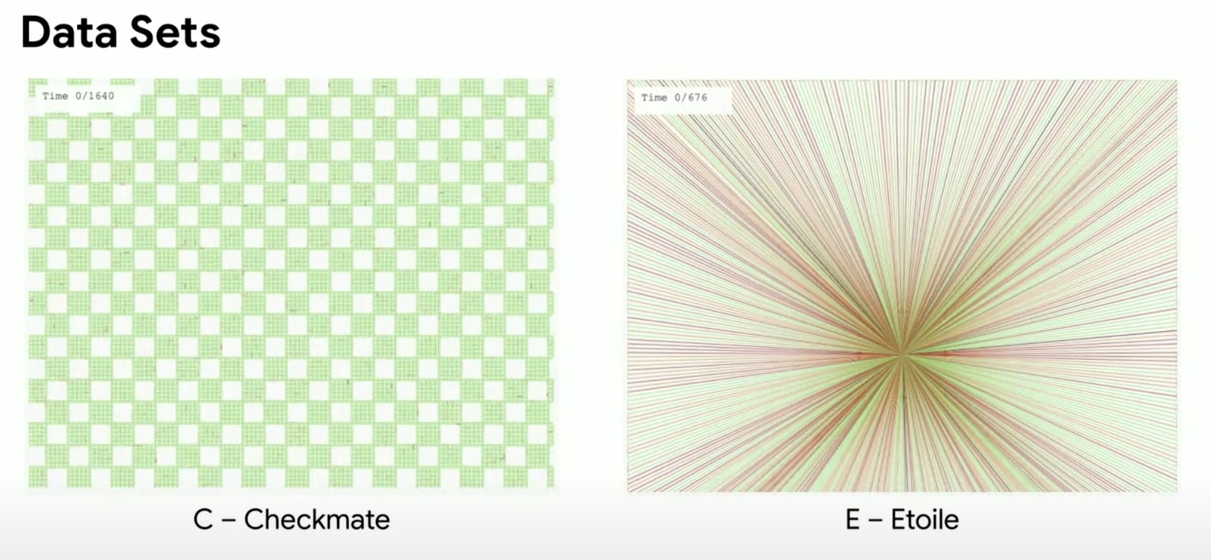
\includegraphics[width=.8\linewidth]{img/screenshots/hashcode_datasets_c_e.png}
    \caption[Visualization of datasets C and E]{
        Visualization of datasets C and E\protect\footnotemark.
    }
    \label{fig:hashcode_dataset_c_e}
    \end{figure}

\footnotetext{\xxx{Screenshot from \href{https://www.youtube.com/watch?v=YPOVd-hQUjA}{Hash Code 2021: Online Qualification Round Livestream}.}}


\section{Simulator} \label{sec:simulator}

This section provides a brief overview of the custom simulator that we developed to serve as a black-box fitness function for the optimization algorithms. We discuss the motivation behind its design and describe the functionality relevant to the optimization process.
\xxx{For further details on the code and implementation, please refer to the Developer documentation in Appendix~\ref{chap:developer_documentation}.}

\bigskip

Our simulator replaces the original competition evaluation system, which was accessible only through the competition website via a user interface and is no longer available. It also adds several features on top of the original system.
The simulator is written in C++ to be as fast and efficient as possible, but is wrapped as a Python package using the powerful pybind11 library~\cite{jakob2017pybind11}, making it very convenient to use.
Inspired by libraries such as NumPy\footnote{\url{https://numpy.org/}} and PyTorch\footnote{\url{https://pytorch.org/}}, our goal is to provide an easy-to-use interface and seamless integration with the vital Python ecosystem, without compromising on top-tier performance.

Below are the features of the simulator package that are important for optimization. These are implemented in C++ and exposed only through a lightweight Python API:
\begin{itemize}
    \item Reading and storing the input data.
    \item Creating initial schedules using several different options.
    \item Running the simulation to evaluate given schedules.
    \item Getting and setting the non-trivial schedules in a format suitable for optimization.
\end{itemize}
The different options for creating initial schedules are described in Section~\ref{sec:initial_schedules} and the format of the non-trivial schedules is described in Section~\ref{sec:coding_of_a_solution}.


The only case where larger data are passed between C++ and Python is when working with the \textit{non-trivial schedules}.
As explained in \hyperref[para:heuristic_2]{Heuristic 2}, these are the only schedules that require optimization.
Since the optimization loop is implemented in Python using parts of the DEAP library~\cite{fortin2012deap}, it must retrieve these schedules from the simulator, modify them externally, and then send the modified schedules back into the simulator to evaluate their score.
